\documentclass[11pt,a4paper]{article}

% --- Encoding & fonts ---
\usepackage[utf8]{inputenc}
\usepackage[T1]{fontenc}
\usepackage{lmodern}
\usepackage{microtype}
\usepackage[english]{babel}

% --- Layout ---
\usepackage[margin=2.2cm]{geometry}
\usepackage{setspace}
\onehalfspacing
\usepackage{parskip}
\setlength{\parindent}{1.2em}
\setlength{\parskip}{0pt plus 1pt}

% --- Math & symbols ---
\usepackage{amsmath,amssymb}
\usepackage{textcomp}
\usepackage{textgreek}

% --- Figures & tables ---
\usepackage{graphicx}
\graphicspath{{figures/}}
\usepackage{booktabs}
\usepackage{array}
\usepackage{multirow}
\usepackage[font=small,labelfont=bf,labelsep=period]{caption}
\usepackage{subcaption}
\usepackage{float}

% --- Citations ---
\usepackage[numbers,sort&compress,square]{natbib}
\bibliographystyle{unsrtnat}

% --- Headings ---
\usepackage{xcolor}
\usepackage{titlesec}
\titleformat{\section}{\normalfont\large\bfseries\color{black!85}}{\thesection}{0.6em}{}
\titleformat{\subsection}{\normalfont\normalsize\bfseries}{\thesubsection}{0.5em}{}

% --- Hyperlinks ---
\usepackage[colorlinks=true,linkcolor=black!70,citecolor=blue!55!black,urlcolor=blue!55!black]{hyperref}

% --- Title block ---
\title{\bfseries\Large Atrial-to-conduction paracrine signaling shapes a\\
spatial maturation gradient in the human fetal heart at PCW12}

\author{%
PantheonOS PCW12 Spatial Analysis Pipeline\\
\textit{Generated report; corresponding workspace:}\\
\texttt{pantheonos-reproducibility/human-heart}%
}
\date{\today}

\begin{document}
\maketitle

% =====================================================================
\begin{abstract}
\noindent
The human cardiac conduction system (CCS) emerges during the first
trimester from a heterogeneous pool of myocytes that must coordinate
their identity with adjacent atrial and ventricular working myocardium.
Whether atrial myocardium (ACM) actively shapes the molecular state of
neighbouring conduction cells in the early fetal heart remains poorly
resolved. Here we use a 100,000-cell three-dimensional MERFISH atlas of
the post-conception week 12 (PCW12) human heart, paired with an entropic
optimal-transport imputation against a matched scRNA-seq reference
\citep{klein2025moscot}, to expand the spatial gene panel from 238 to
5{,}187 genes and recover a genome-scale spatial cell--cell interactome
using Spateo \citep{qiu2024spateo}. Re-running the analysis with this
expanded panel grew the testable ligand--receptor (LR) catalogue from
$\sim$11 to 388 pairs and revealed 159 spatially significant interactions
spanning neuregulin--ErbB, ECM--integrin, Eph--ephrin and semaphorin
modules. Focusing on the conduction compartment, ACM-derived NRG3 and
SEMA3A emerge as the dominant inputs to core conduction cells (CCC).
A nearest-neighbour spatial test confirmed that NRG3 expression in ACM
and ERBB4 expression in adjacent CCC are spatially coupled
($\rho{=}+0.22$, $p_{\text{perm}}{<}10^{-3}$). Unsupervised clustering of
the 292 CCC on a curated receptor and CCS-transcription-factor panel
resolved seven transcriptional subtypes with clearly interpretable
signatures, including an AV-node-like (TBX2/TBX3$^+$), SAN-like
(SHOX2$^+$ NKX2-5$^+$) and TBX18$^+$ sinus-venosus subset. Across the
full CCC pool, ACM-niche scores for NRG3 and SEMA3A were systematically
\emph{negatively} correlated with conduction-system transcription
factors (NKX2-5, TBX3, TBX5, SHOX2, TBX18; FDR ${\le}10^{-3}$). Together,
the data support a model in which proximity to atrial paracrine input
sustains a less-differentiated CCC pool while specified pacemaker, AV
node and sinus-venosus-derived cells reside further from the source.
\end{abstract}

\vspace{0.6em}
\noindent\textbf{Keywords:} cardiac conduction system; spatial
transcriptomics; MERFISH; optimal transport; cell--cell interaction;
neuregulin; ErbB4; SEMA3A; TBX3; SHOX2.

% =====================================================================
\section{Introduction}

The cardiac conduction system (CCS) --- comprising the sinoatrial node
(SAN), the atrioventricular node (AVN), the bundle of His and the
Purkinje fibre network --- is responsible for orchestrating the
sequential contraction of the four chambers of the heart. Its
morphogenesis begins early in cardiac development from heterogeneous
progenitor pools, and aberrations of this process underlie a substantial
fraction of congenital arrhythmias and conduction
disorders~\citep{vanweerd2016ccsreview,park2017ccs}. Decades of mouse
genetics have established a core transcriptional network governing CCS
specification and function: \emph{Tbx3} is required for the SAN/AVN gene
program~\citep{hoogaars2007tbx3}; \emph{Shox2} represses
\emph{Nkx2-5} in the sinus venosus to permit pacemaker
identity~\citep{espinozalewis2009shox2,blaschke2007shox2}; \emph{Tbx18}
defines the head of the SAN and venous pole
\citep{christoffels2006tbx18,wiese2009tbx18tbx3}; and the funny current
generated by HCN channels confers spontaneous diastolic depolarisation
to pacemaker cells~\citep{difrancesco2010funny}.

In parallel, ligand--receptor signalling has been shown to shape CCS
differentiation. Neuregulin--ErbB signalling is essential for cardiac
development~\citep{lee1995erbb2,meyer1995neuregulin}; conditional
loss-of-function studies further established that NRG-1 promotes
formation of the murine cardiac conduction
system~\citep{rentschler2002nrg1ccs}, and SEMA3A is required for normal
cardiac rhythm by patterning sympathetic
innervation~\citep{ieda2007sema3a}. However, almost all of this
mechanistic knowledge derives from mouse models or in-vitro systems.
The corresponding paracrine architecture in the early human fetal heart
--- where the conducting compartment is intimately interleaved with
working myocardium and contains multiple molecularly distinct subtypes
--- has been difficult to resolve because the available spatial
technologies sacrifice gene breadth for spatial resolution.

Recent advances in image-based spatial transcriptomics
\citep{chen2015merfish,moffitt2018merfish} and 3D spatiotemporal modelling
\citep{qiu2024spateo} now enable cell-resolution interrogation of intact
human organs, but at the cost of restricted gene panels (typically
$\lesssim$300 genes) that exclude most ligand--receptor pairs. Optimal
transport (OT) provides a principled remedy: by aligning a high-content
scRNA-seq reference to a spatial sample in an entropically regularised
coupling, OT permits gene imputation onto unmeasured genes
\citep{schiebinger2019wot,klein2025moscot}.

In this report we apply this strategy to a 100{,}000-cell 3D MERFISH
atlas of the human heart at PCW12, paired with a stage-matched scRNA-seq
reference. Imputing $\sim$5{,}000 highly variable genes plus a curated
heart-disease gene panel multiplies the testable LR landscape by
$\sim$35-fold and reveals dominant atrial-to-conduction paracrine axes
that are absent from the panel-restricted analysis. We then validate
the strongest axis (NRG3$\to$ERBB4) with a spatial nearest-neighbour
test, dissect heterogeneity within the core conduction compartment, and
demonstrate that proximity to ACM-derived ligands is anti-correlated
with CCS transcription factor expression --- pointing to a niche-driven
maturation gradient.

% =====================================================================
\section{Results}

\subsection{Expanded MOSCOT imputation enables genome-scale spatial CCI}
\label{sec:imputation}

The MERFISH panel measures 238 genes across 100{,}000 cells in 3D, of
which only $\sim$60 overlap the Spateo human ligand--receptor database;
direct application of cell--cell interaction analysis yielded merely
$\sim$11 testable LR pairs and a single biological axis (DLL4--NOTCH2).
To overcome this, we used the entropic OT framework
\textsc{moscot}~\citep{klein2025moscot} to map a stage-matched PCW12
scRNA-seq atlas (32{,}870 cells $\times$ 31{,}019 genes) onto the
spatial sample (Methods). The mapping was performed in five batches of
$2 \times 10^4$ spatial cells against the full SC reference, with
local-PCA-based costs and asymmetric marginals
($\tau_a{=}1, \tau_b{=}0.9$). Imputation used the union of the top
5{,}000 highly variable genes (HVGs) and a curated panel of 247 heart
disease genes, intersected with the SC reference, yielding 5{,}187
imputed genes per spatial cell.

Coverage of the Spateo LR database increased from 2 ligands and 3
receptors (panel-only) to 185 and 189 respectively, expanding the
testable ordered LR catalogue from $\sim$11 to 388 (Table~\ref{tab:cov}).
Re-running the Spateo \texttt{find\_cci\_two\_group} analysis on a
20{,}000-cell stratified subsample across the eight largest cell types
(ACM, VCM, FB, Endocardial, MuralCells, NC, CoreConductionCells,
TzConductionCells) returned non-empty results for all 56 ordered cell
type pairs and flagged 159 LR rows as significant
(Figure~\ref{fig:f1}c). The recovered interactome spans the canonical
modules of fetal cardiogenesis --- neuregulin--ErbB (cardiomyocyte
proliferation), collagen and laminin--integrin (basement membrane and
matrix--stroma), Eph--ephrin (boundary formation), semaphorin--plexin
(guidance) and PDGF (pericyte recruitment).

\begin{table}[H]
\centering
\caption{LR-database coverage before and after gene-set expansion.}
\label{tab:cov}
\small
\begin{tabular}{lrr}
\toprule
Metric & Panel only (238 g) & \textbf{Imputed (5{,}187 g)} \\
\midrule
Spateo ligands present       & 2  & \textbf{185} \\
Spateo receptors present     & 3  & \textbf{189} \\
Testable ordered LR pairs    & $\sim$11 & \textbf{388} \\
Cell-type pairs returning data & 5/56 & \textbf{56/56} \\
Significant LR rows (top-3 / pair) & 5 & \textbf{159} \\
Distinct biological axes     & 1  & $>$10 \\
\bottomrule
\end{tabular}
\end{table}

\begin{figure}[!htbp]
\centering
\begin{subfigure}[t]{0.45\linewidth}
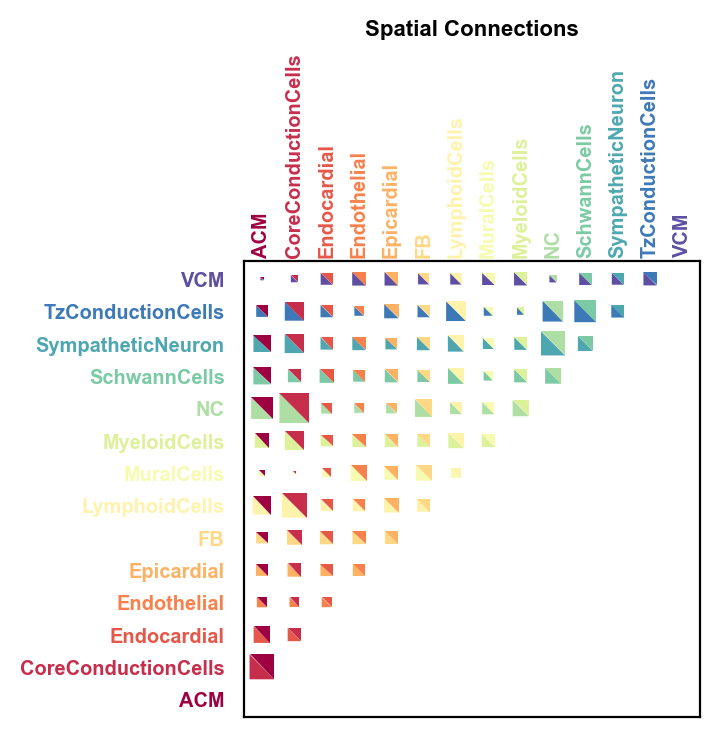
\includegraphics[width=\linewidth]{F1a_connectivity.png}
\caption{Cell-type connectivity matrix.}
\end{subfigure}\hfill
\begin{subfigure}[t]{0.50\linewidth}
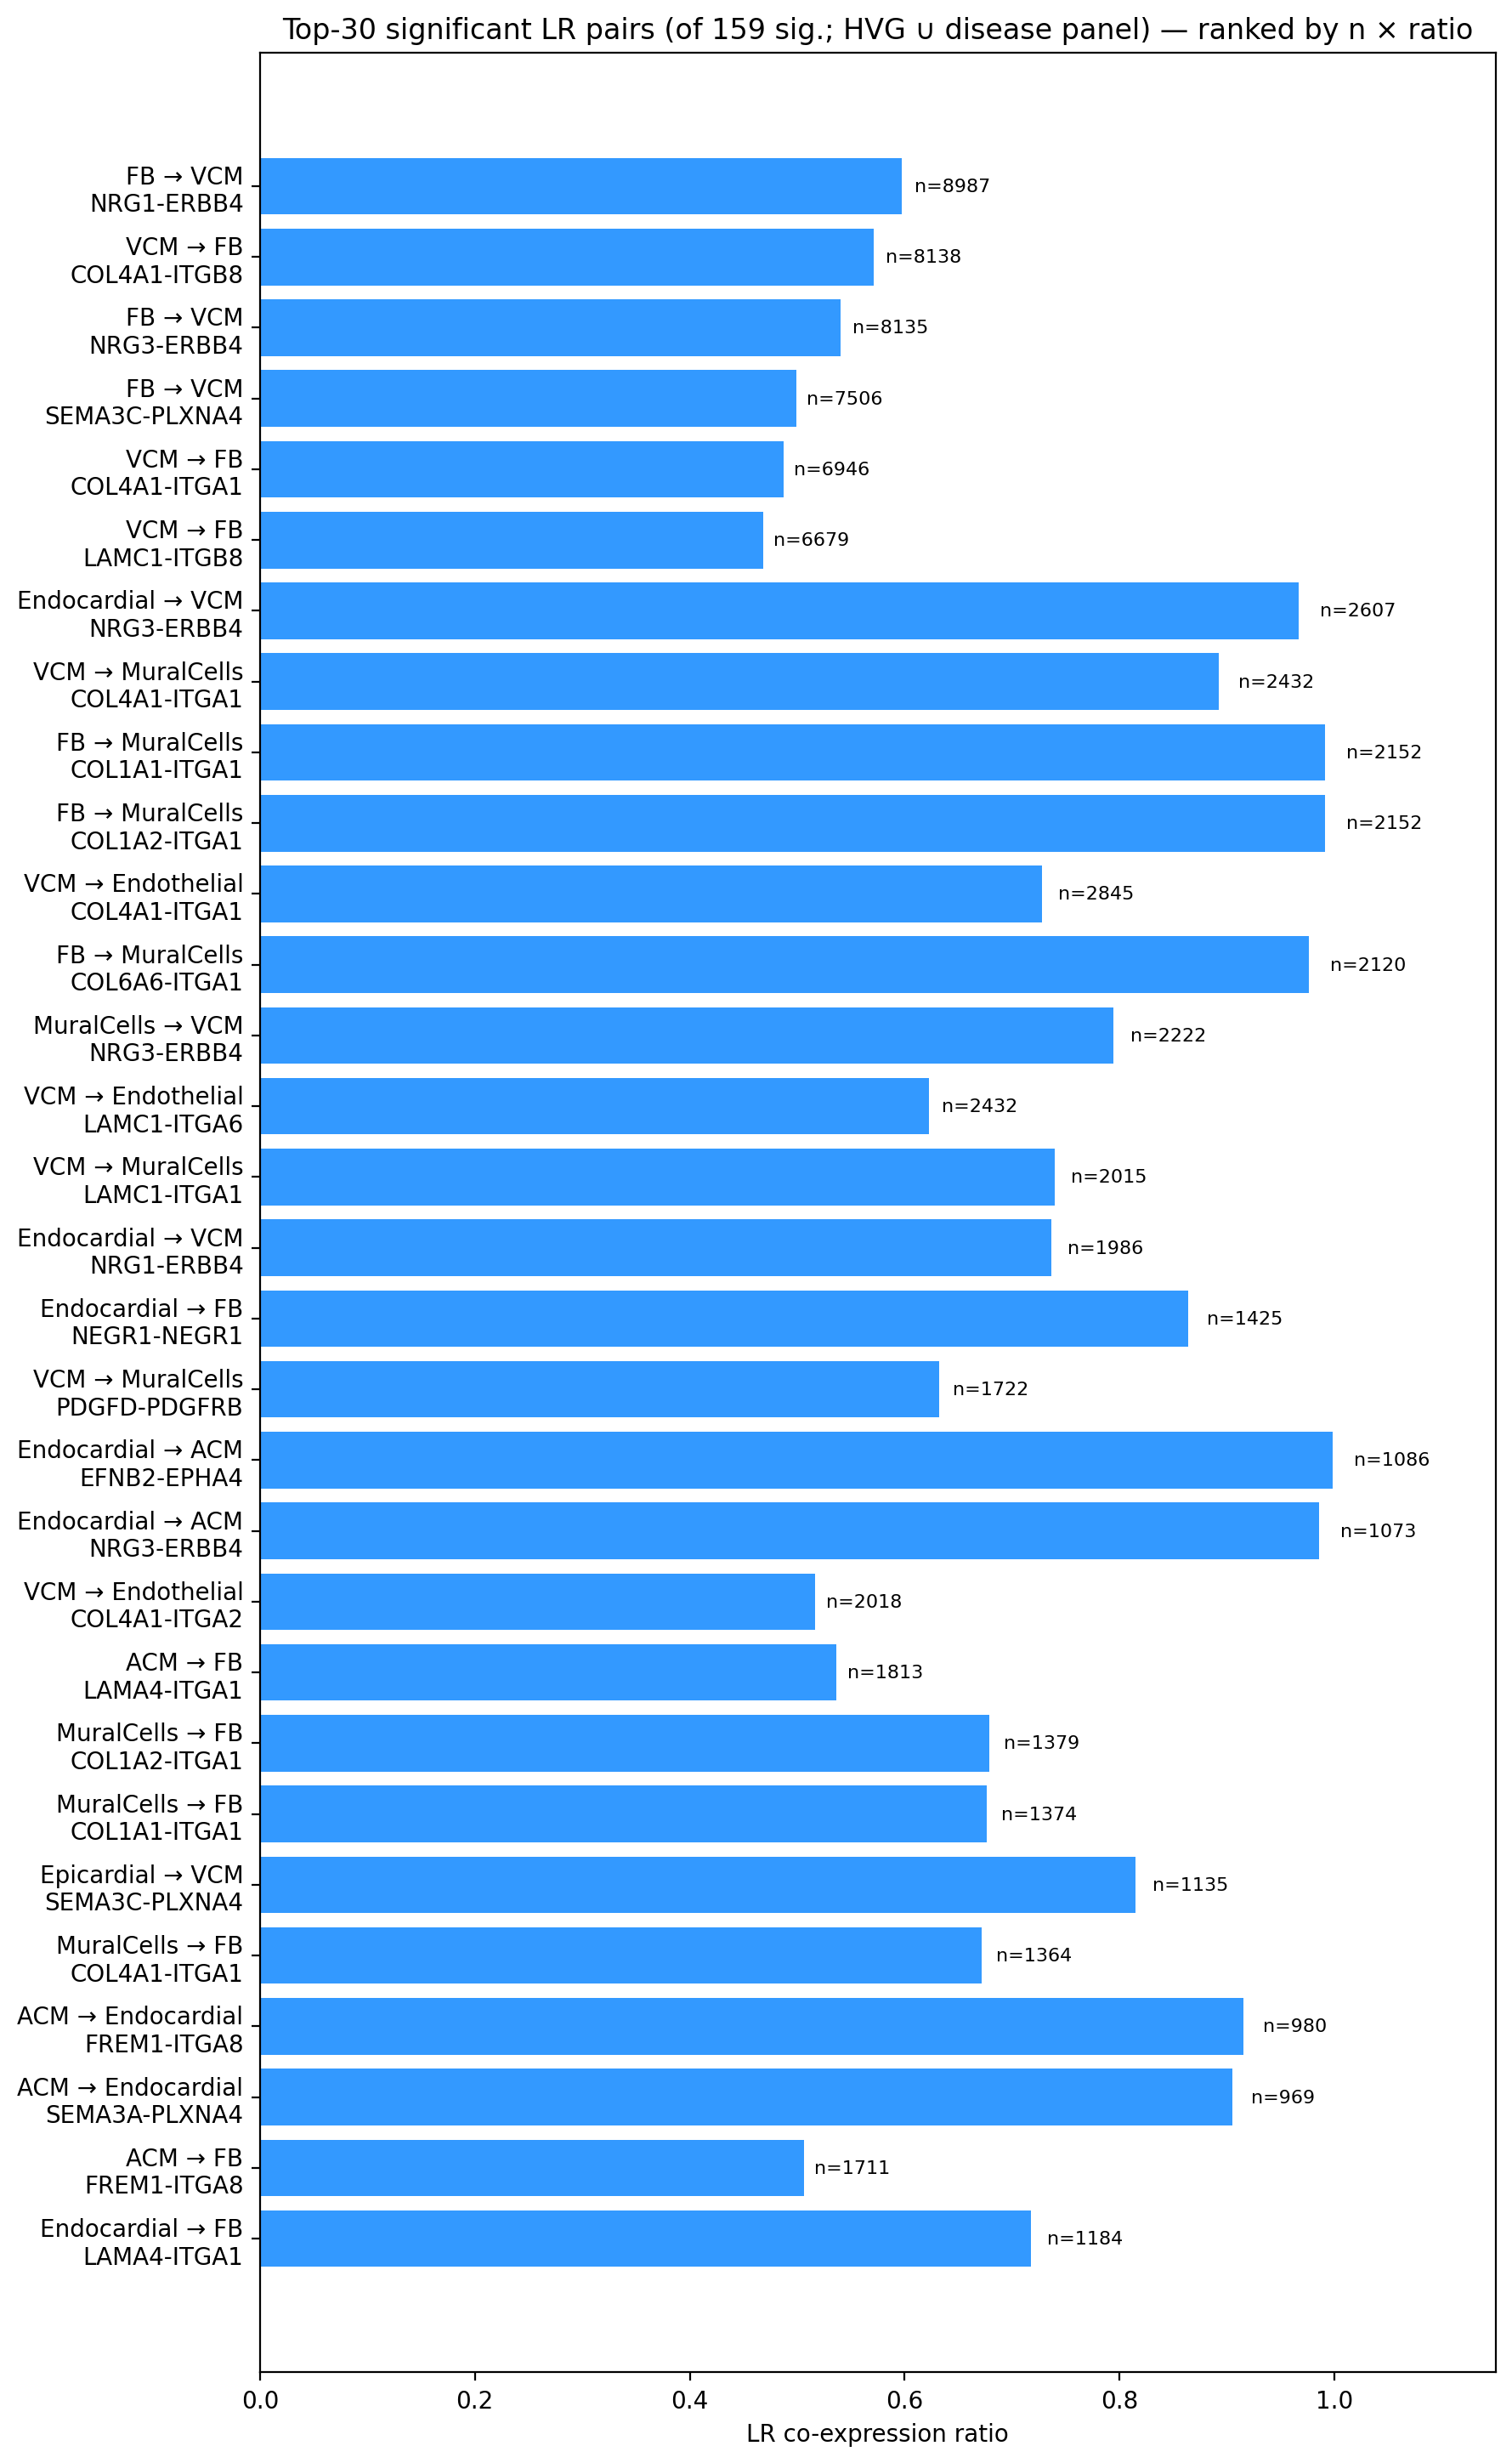
\includegraphics[width=\linewidth]{F1c_overview.png}
\caption{Top significant LR pairs across 56 cell-type pairs.}
\end{subfigure}
\caption{\textbf{Genome-scale spatial cell--cell interactome of the
PCW12 heart.} (a)~Cell-type connectivity matrix derived from the
Spateo k-NN graph on the 20{,}000-cell stratified subsample; entries
report the number of inter-cell-type contacts. (b)~Top 30
significant ligand--receptor pairs across the 56 ordered cell-type
pairs, ranked by spatial co-expression count. Bar height is the
number of co-expressing cell pairs ($n$); grey opacity encodes the
co-expression ratio. Pairs are coloured by sender--receiver identity.}
\label{fig:f1}
\end{figure}

\subsection{Atrial myocardium signals to core conduction cells via
NRG3 and SEMA3A}
\label{sec:acm-ccc}

Focusing on the conducting compartment, we ran Spateo
\texttt{find\_cci\_two\_group} on six ordered pairs centred on
\texttt{CoreConductionCells} (CCC) and its immediate neighbours
\texttt{ACM}, \texttt{NC} (neural crest) and
\texttt{TzConductionCells}, with $N_{\text{perm}}{=}50$. Across the
ACM$\to$CCC pair (the most populated of the six), 18 LR pairs reached
significance. The two strongest signals were
\textbf{NRG3--ERBB4} ($n{=}79$ co-expressing cell pairs, ratio 0.44) and
\textbf{SEMA3A--PLXNA4} ($n{=}71$, ratio 0.40)
(Figure~\ref{fig:f2}a). The NRG3--ERBB4 axis is the spatial-omics
correlate of an interaction with deep developmental support: NRG-1 has
been shown to promote murine CCS formation in vivo
\citep{rentschler2002nrg1ccs} and the wider NRG/ErbB axis is required
for cardiogenesis in mice \citep{lee1995erbb2,meyer1995neuregulin}.
SEMA3A is required for normal cardiac
rhythm in vivo \citep{ieda2007sema3a}; its appearance here as the
second-strongest ACM$\to$CCC signal at PCW12 is consistent with a
guidance / repulsion role in shaping the AV junction.

The reverse direction (CCC$\to$ACM) yielded only six significant pairs,
dominated by EFNB2--EPHA4, FGF10--FGFR2 and BMP4--BMPR2; signalling is
therefore strongly asymmetric, with ACM as the dominant sender. An
analogous analysis of the NC$\to$CCC pair recovered the canonical
neural-crest$\to$conduction-system signal SEMA3C--PLXNA4 (ratio 0.75)
and a bidirectional COL1/COL4--integrin ECM axis
(Figure~\ref{fig:f2}b). The TzConductionCells--CCC pair was largely
silent, likely reflecting both the small population of transitional
cells in the subsample and limited contact between the two compartments
at this developmental stage.

\begin{figure}[!htbp]
\centering
\begin{subfigure}[t]{0.42\linewidth}
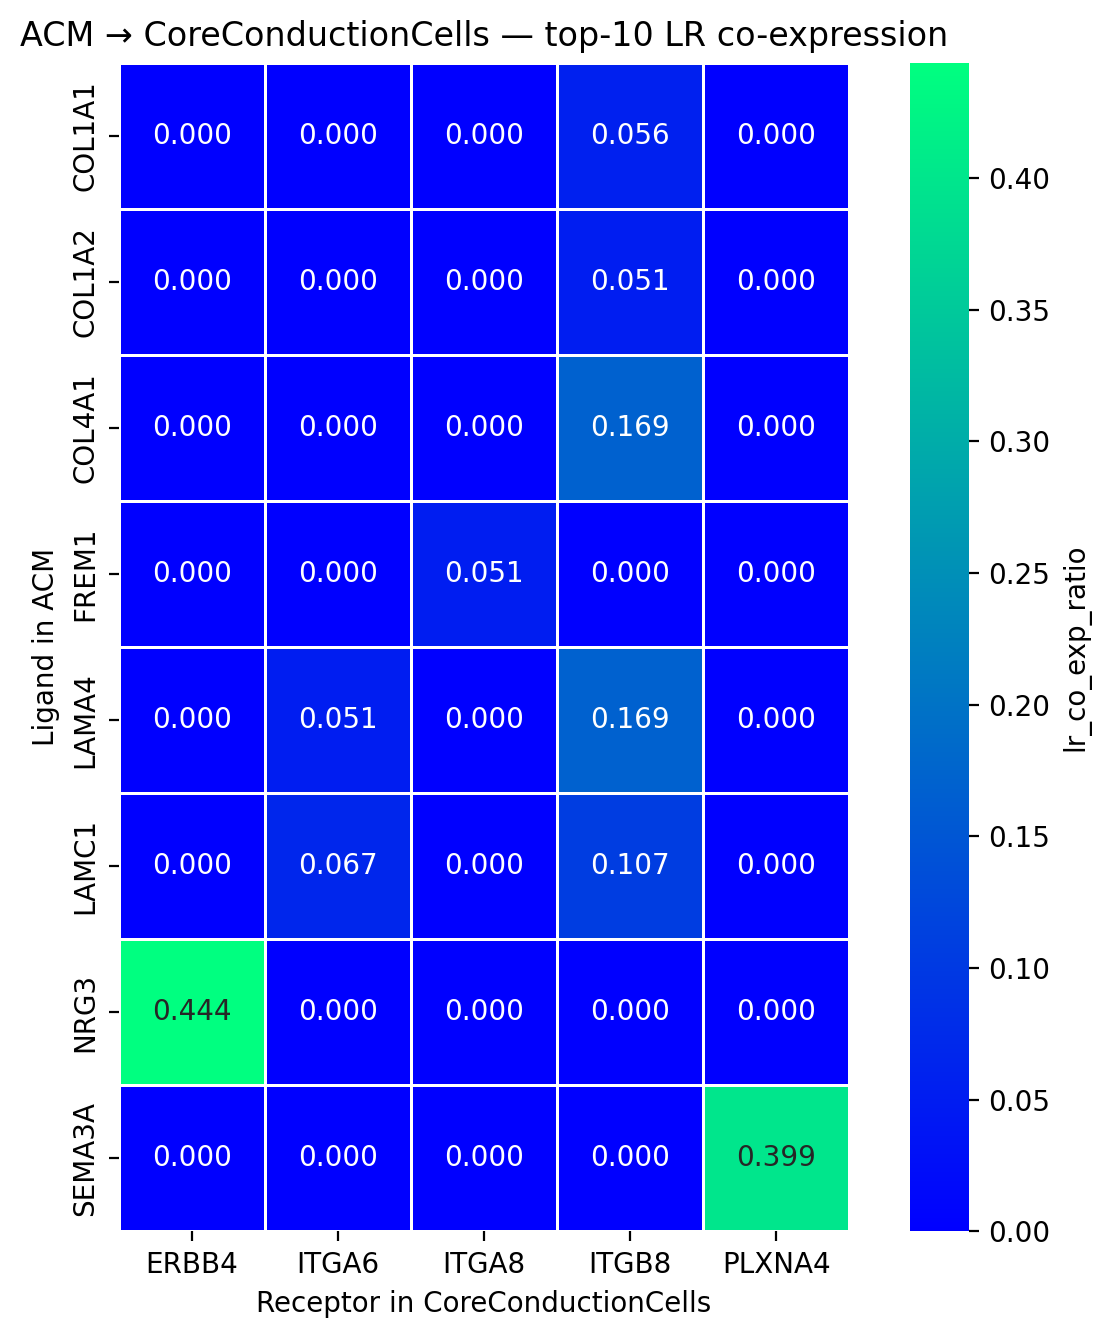
\includegraphics[width=\linewidth]{F2a_ACM_CCC_heatmap.png}
\caption{ACM $\to$ CCC}
\end{subfigure}\hfill
\begin{subfigure}[t]{0.42\linewidth}
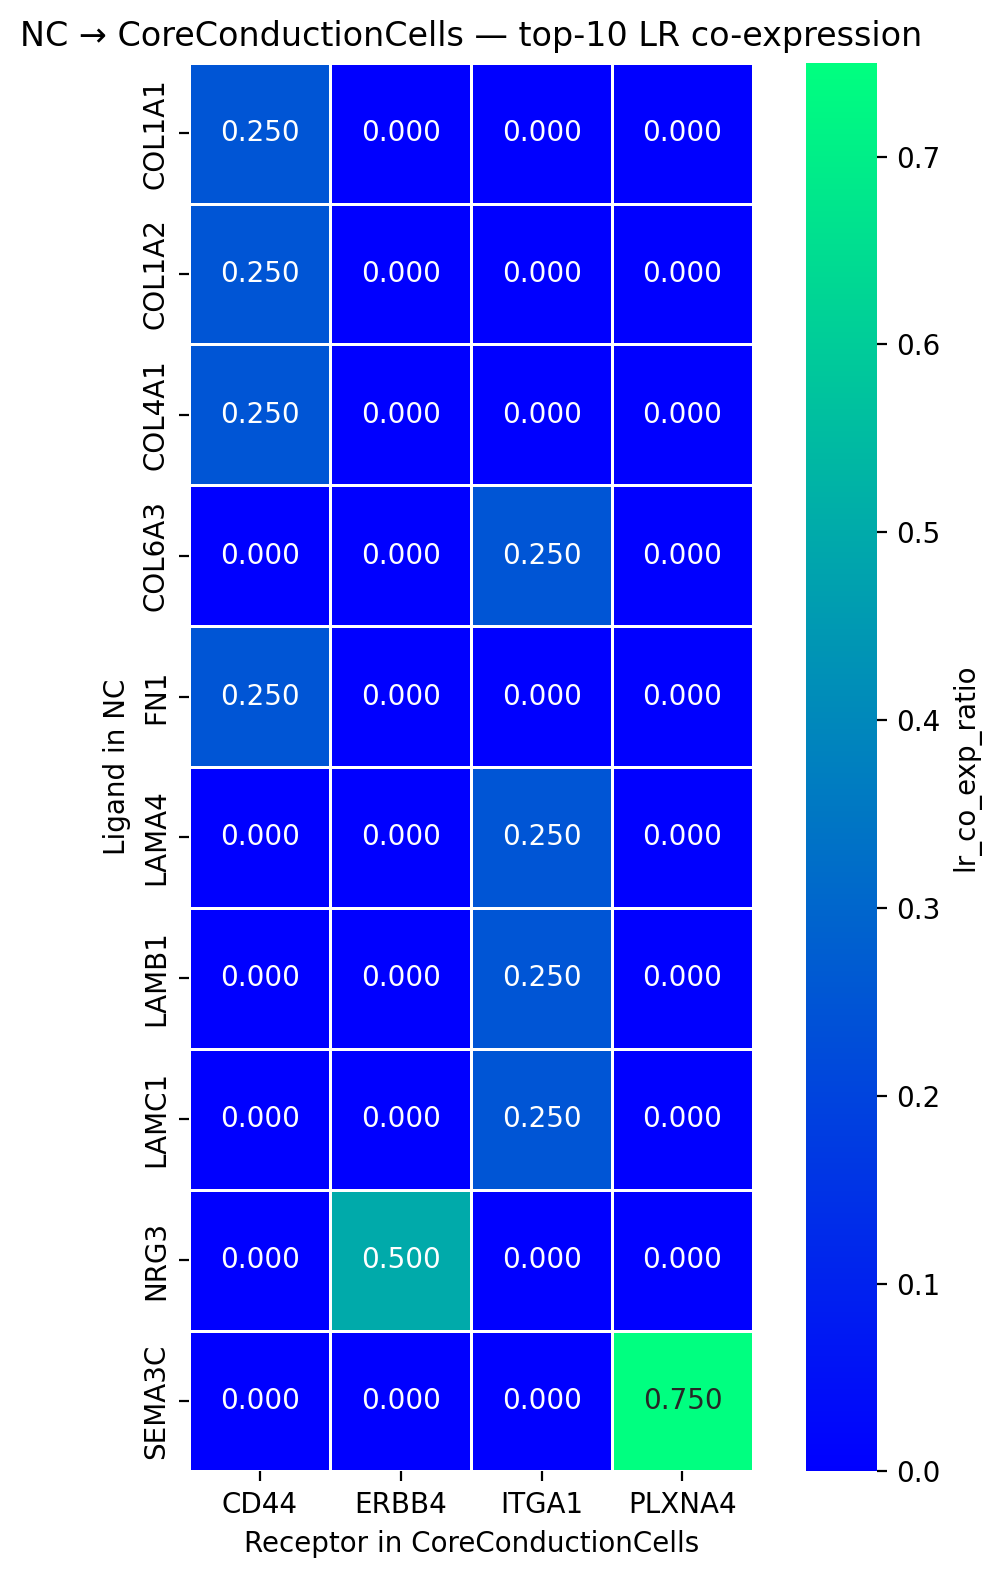
\includegraphics[width=\linewidth]{F2b_NC_CCC_heatmap.png}
\caption{NC $\to$ CCC}
\end{subfigure}\\[0.4em]
\begin{subfigure}[t]{0.62\linewidth}
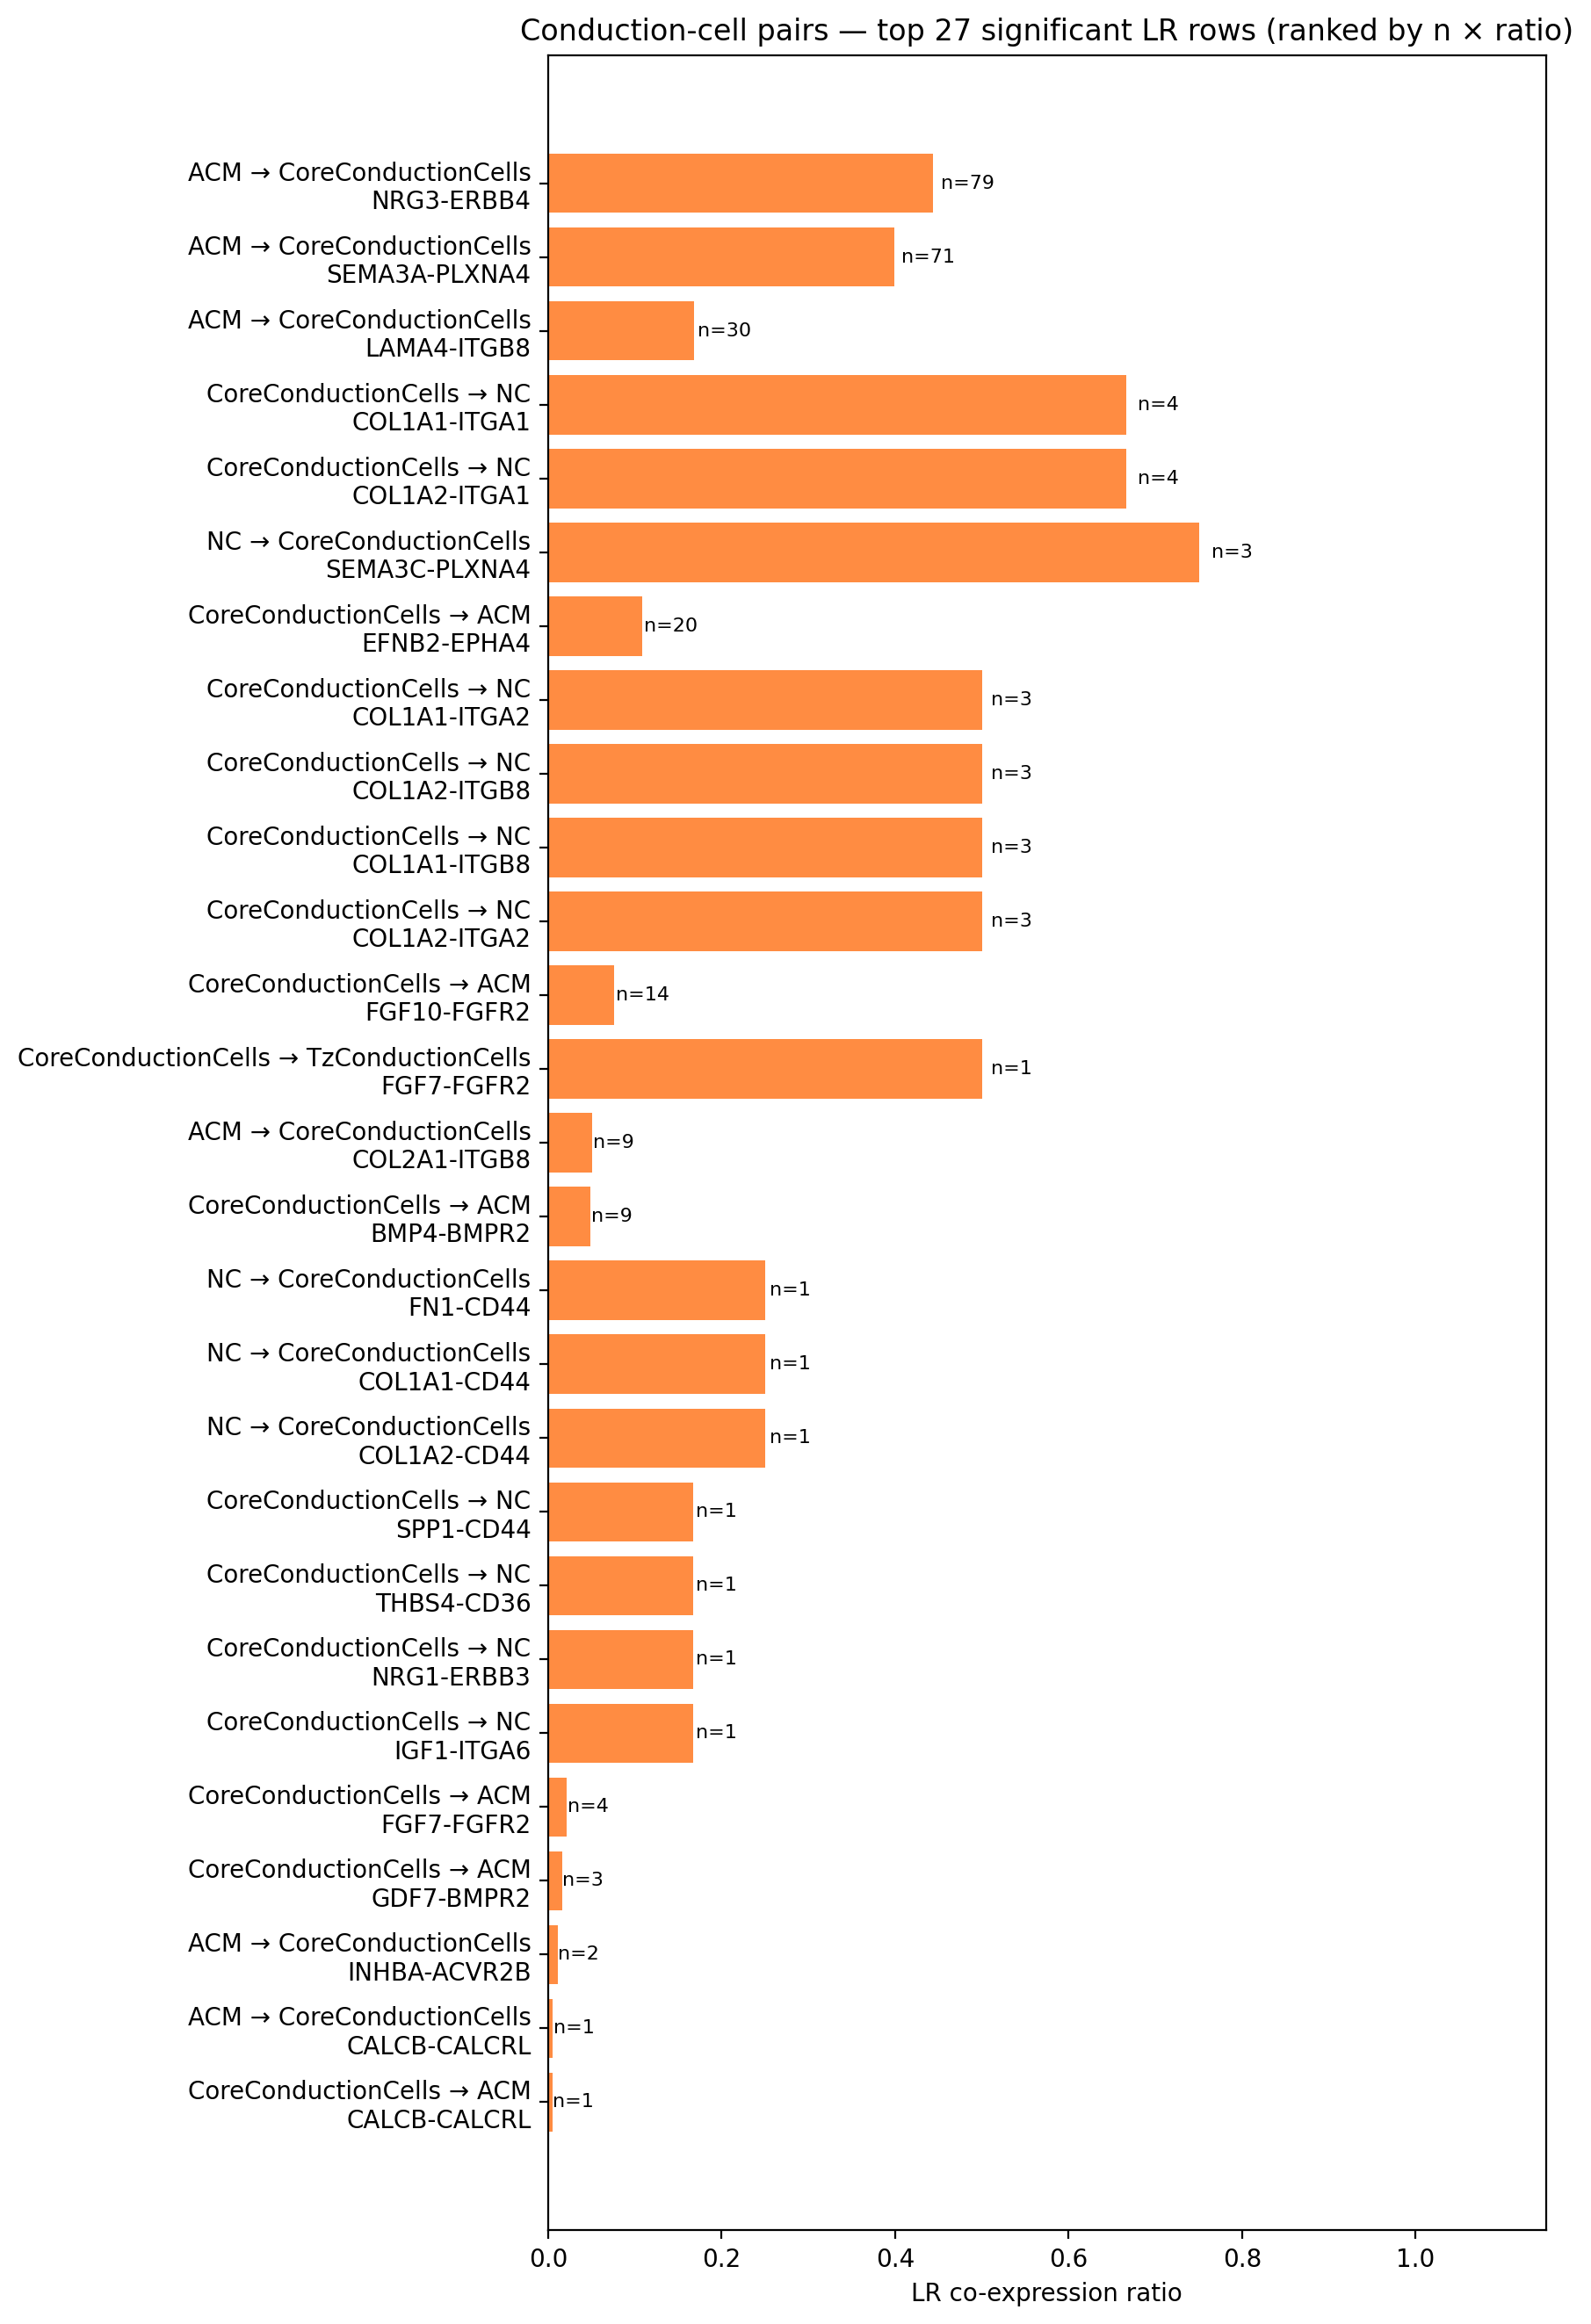
\includegraphics[width=\linewidth]{F2c_conduction_overview.png}
\caption{Conduction-pair overview: significant LR pairs across all six
CCC-centred ordered pairs. NRG3--ERBB4 and SEMA3A--PLXNA4 dominate the
ACM$\to$CCC axis.}
\end{subfigure}
\caption{\textbf{ACM and NC are the dominant senders of paracrine
input to CCC.} Heatmaps show LR-pair significance scores across the
top hits per pair; opacity encodes the co-expression ratio.}
\label{fig:f2}
\end{figure}

\subsection{NRG3$\to$ERBB4 paracrine coupling is spatially coherent}
\label{sec:nrg3erbb4}

A high LR co-expression count is necessary but not sufficient evidence
for paracrine coupling: ligand and receptor could be expressed at the
right ratios in the right cell types yet not be \emph{spatially
adjacent}. To test for spatial coherence, we returned to the full
imputed atlas (CCC $n{=}292$, ACM $n{=}9{,}955$) and, for each CCC cell,
recorded the ligand expression (NRG3 or SEMA3A) of its single nearest
ACM neighbour in 3D. We then computed Spearman correlation against the
CCC cell's receptor (ERBB4 or PLXNA4) and assessed significance against
a 1{,}000-permutation null in which CCC--ACM pairings were randomly
re-shuffled (Methods).

The NRG3$\to$ERBB4 axis showed a clean positive correlation
($\rho{=}+0.219$, $p_{\text{perm}}{<}10^{-3}$) that fell well outside
the permutation null (range $\pm 0.13$; Figure~\ref{fig:f3}b). The
SEMA3A$\to$PLXNA4 axis was significantly \emph{negative}
($\rho{=}-0.121$, $p_{\text{perm}}{=}0.037$): PLXNA4-high CCC sit
\emph{further} from SEMA3A-high ACM, consistent with the known
repulsive guidance function of class-3 semaphorins. Three-dimensional
visualisation of ACM and CCC populations confirmed that ERBB4-high CCC
preferentially occupy regions adjacent to NRG3-high ACM, while PLXNA4
expression in CCC was spatially less structured
(Figure~\ref{fig:f3}a,c).

\begin{figure}[!htbp]
\centering
\begin{subfigure}[t]{0.78\linewidth}
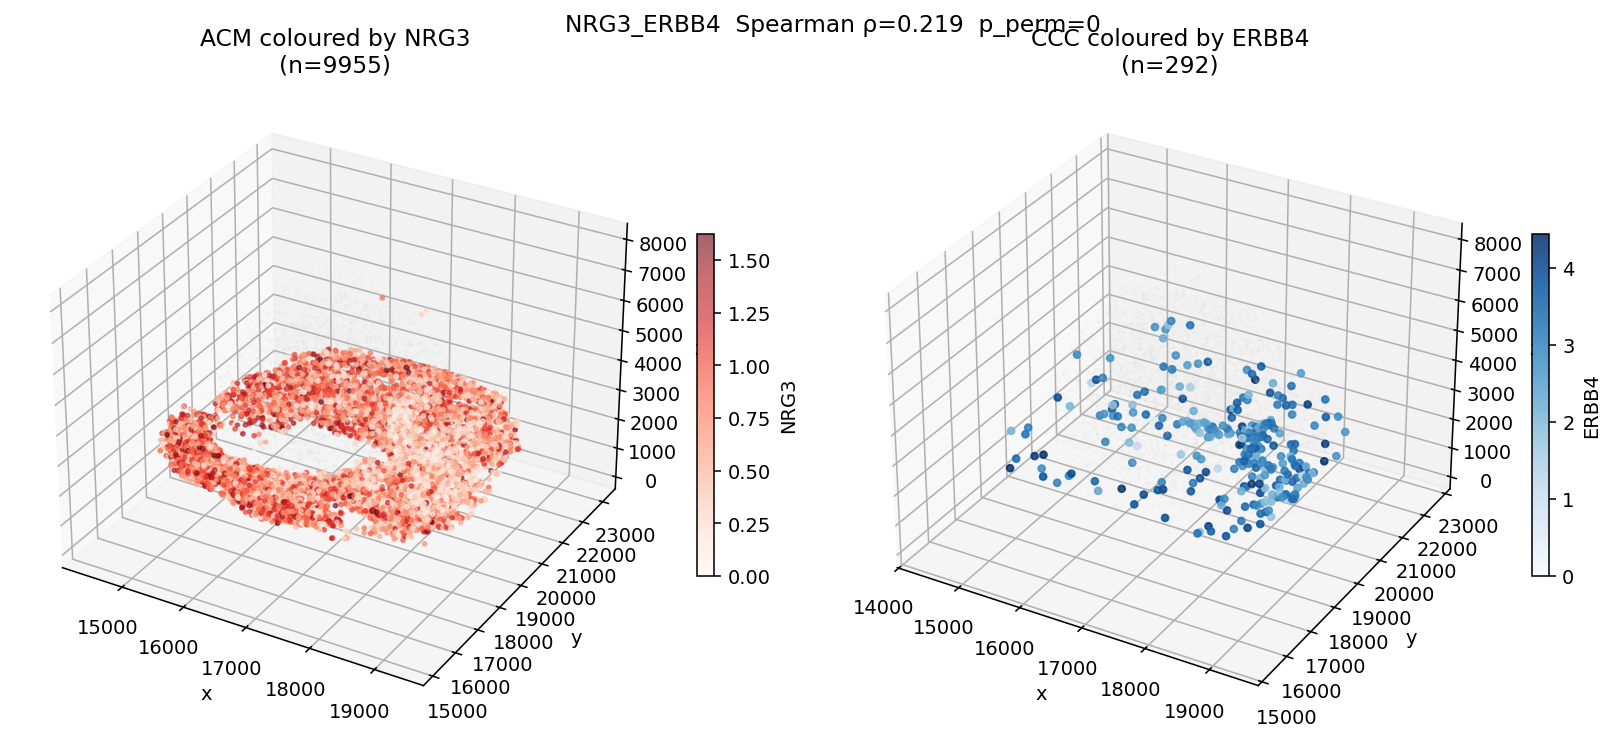
\includegraphics[width=\linewidth]{F3a_NRG3_ERBB4_3d.png}
\caption{NRG3 in ACM and ERBB4 in CCC, 3D coordinates.}
\end{subfigure}\\[0.4em]
\begin{subfigure}[t]{0.40\linewidth}
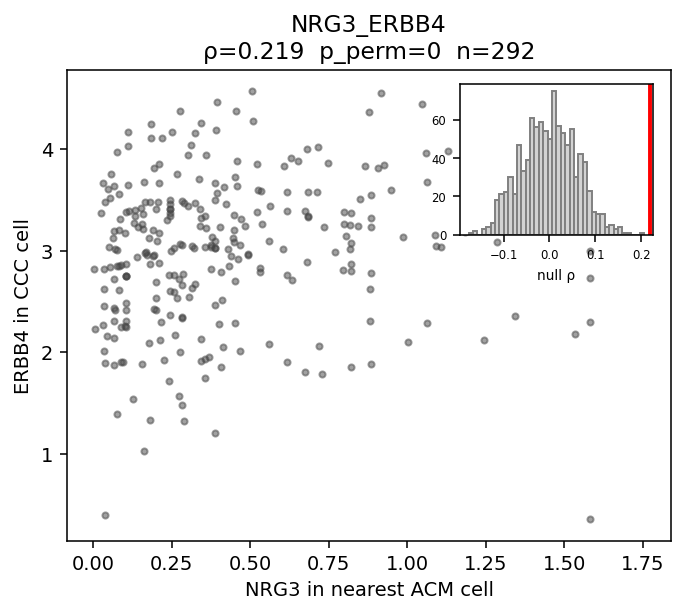
\includegraphics[width=\linewidth]{F3b_NRG3_ERBB4_scatter.png}
\caption{Spearman scatter and permutation null inset.}
\end{subfigure}\hfill
\begin{subfigure}[t]{0.55\linewidth}
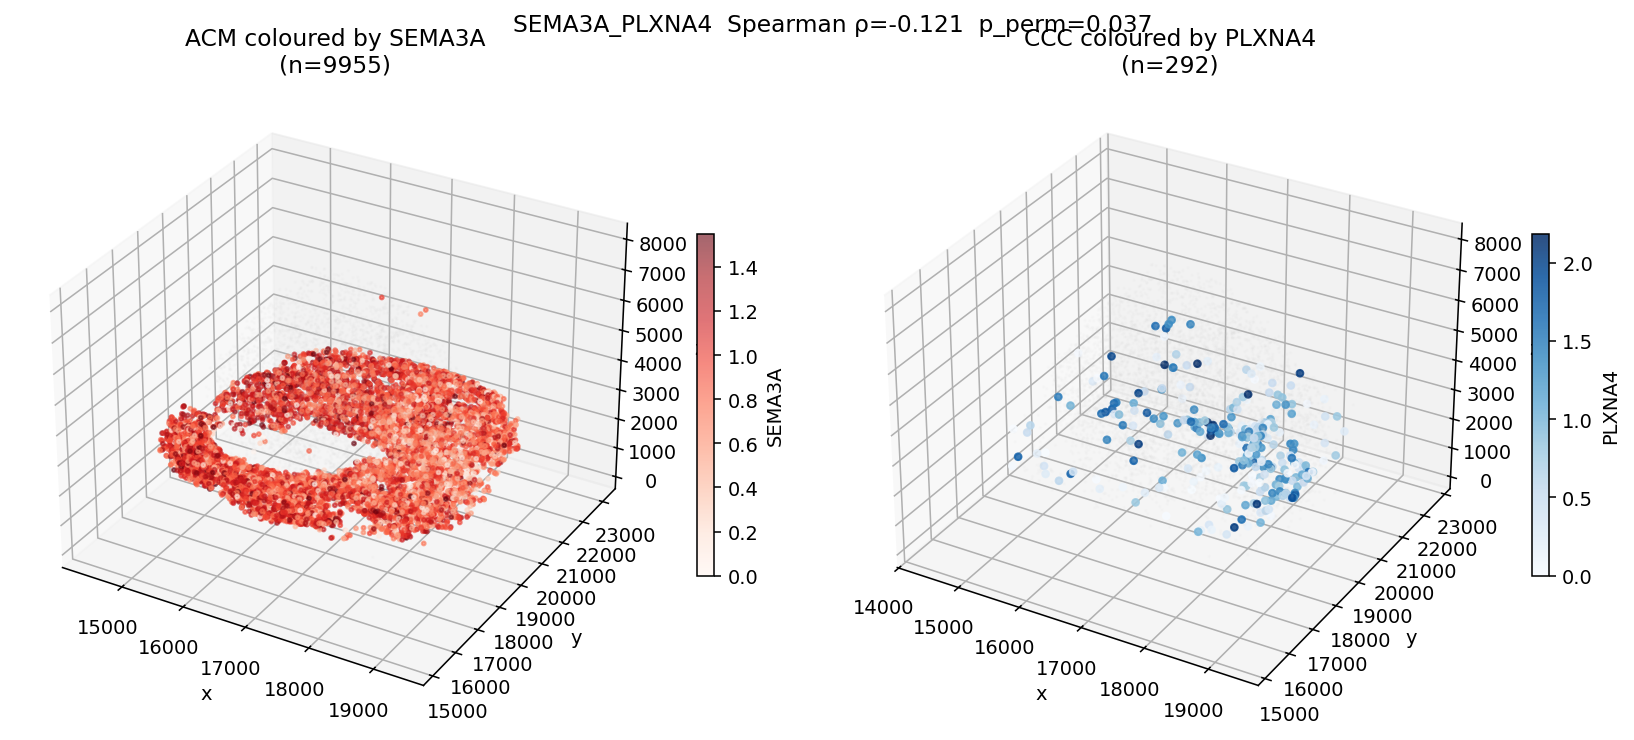
\includegraphics[width=\linewidth]{F3c_SEMA3A_PLXNA4_3d.png}
\caption{SEMA3A--PLXNA4 axis (negative coupling).}
\end{subfigure}
\caption{\textbf{Spatial validation of paracrine coupling.}
The NRG3$\to$ERBB4 axis is positively coupled in space; the
SEMA3A$\to$PLXNA4 axis is significantly anti-coupled, consistent with
semaphorin's repulsive role.}
\label{fig:f3}
\end{figure}

\subsection{Core conduction cells partition into seven transcriptional
subtypes recovering canonical CCS biology}
\label{sec:heterogeneity}

A single \texttt{CoreConductionCells} label on the spatial atlas masks
substantial molecular heterogeneity. To dissect this, we extracted the
full set of 292 CCC cells from the imputed atlas and re-clustered them
on a curated panel of 8 receptors (ERBB3, ERBB4, FGFR2, PLXNA4, EPHA4,
ITGA1, ITGB8, BMPR2) and 10 CCS transcription factors (TBX3, TBX5,
TBX18, TBX2, NKX2-5, ISL1, SHOX2, HCN1, GJA5, GJA1). Note that HCN4 and
CNTN2 were not retained in the 5{,}187-HVG imputed set; HCN1 was used
as the closest available pacemaker-channel surrogate (also expressed
in His--Purkinje tissue). After Scanpy preprocessing (PCA, neighbour
graph) \citep{wolf2018scanpy}, Leiden community
detection~\citep{traag2019leiden} returned seven subclusters
(Figure~\ref{fig:f4}a) with clearly interpretable
signatures (Figure~\ref{fig:f4}c, Table~\ref{tab:ccc-subtypes}).

\begin{table}[H]
\centering
\caption{CCC subclusters and their inferred CCS-subtype identity.}
\label{tab:ccc-subtypes}
\small
\begin{tabular}{rrlp{6.4cm}}
\toprule
Cluster & $n$ & Signature & Inferred identity / supporting refs \\
\midrule
\textbf{c1} & 51 & HCN1$\uparrow$ GJA5$\uparrow$ FGFR2$\uparrow$ &
Pacemaker / conducting (canonical
HCN$^+$~\citep{difrancesco2010funny}; GJA5$^+$) \\
\textbf{c2} & 49 & TBX2$\uparrow$ TBX3$\uparrow$ EPHA4$\uparrow$ &
AV-node-like (TBX3 imposes pacemaker
program~\citep{hoogaars2007tbx3}) \\
\textbf{c6} & 16 & SHOX2$\uparrow$ NKX2-5$\uparrow$ BMPR2$\uparrow$ &
SAN-like (SHOX2 is the SAN master
regulator~\citep{espinozalewis2009shox2,blaschke2007shox2}) \\
\textbf{c5} & 26 & TBX18$\uparrow$ ALDH1A2$\uparrow$ &
Sinus-venosus / pro-epicardial origin
\citep{christoffels2006tbx18,wiese2009tbx18tbx3} \\
\textbf{c3} & 48 & ISL1$\uparrow$ GJA1$\uparrow$ &
Transitional / atrial--CCS border \\
c0 & 66 & ERBB3$\uparrow$ ITGA1$\uparrow$ ALCAM$\uparrow$ &
ECM / vascular-niche subset \\
c4 & 36 & low everything; MRC2$\uparrow$ FKTN$\uparrow$ &
Poorly-differentiated / fibrotic-niche \\
\bottomrule
\end{tabular}
\end{table}

The five biologically labelled clusters (c1, c2, c3, c5, c6) account
for $\sim$65\% of the CCC pool. The recovery of an AV-node-like
(TBX2$^+$/TBX3$^+$/EPHA4$^+$), a SAN-like
(SHOX2$^+$/NKX2-5$^+$/BMPR2$^+$) and a TBX18$^+$ sinus-venosus subset
within a single un-curated annotation label demonstrates that the
imputed receptor + TF panel is sufficient to discriminate canonical CCS
subtypes from spatial-omics data alone. Three-dimensional spatial
positions of the seven subclusters were largely intermingled
(Figure~\ref{fig:f4}b), indicating that no clean
anatomical regionalisation of these subtypes is detectable at this
developmental stage and resolution. Whether this is a real
developmental feature of the PCW12 heart or an artefact of MERFISH
cell-type label mixing remains to be resolved with orthogonal data.

\begin{figure}[!htbp]
\centering
\begin{subfigure}[t]{0.45\linewidth}
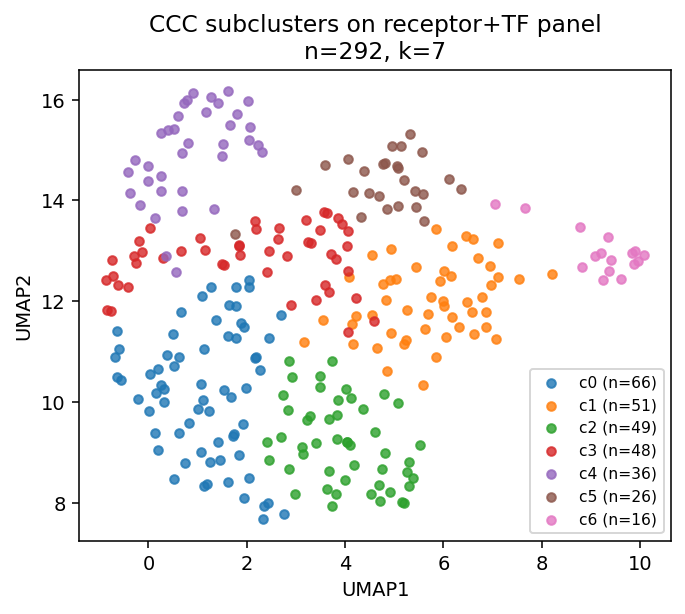
\includegraphics[width=\linewidth]{F4a_ccc_umap.png}
\caption{UMAP of 292 CCC, coloured by Leiden cluster.}
\end{subfigure}\hfill
\begin{subfigure}[t]{0.45\linewidth}
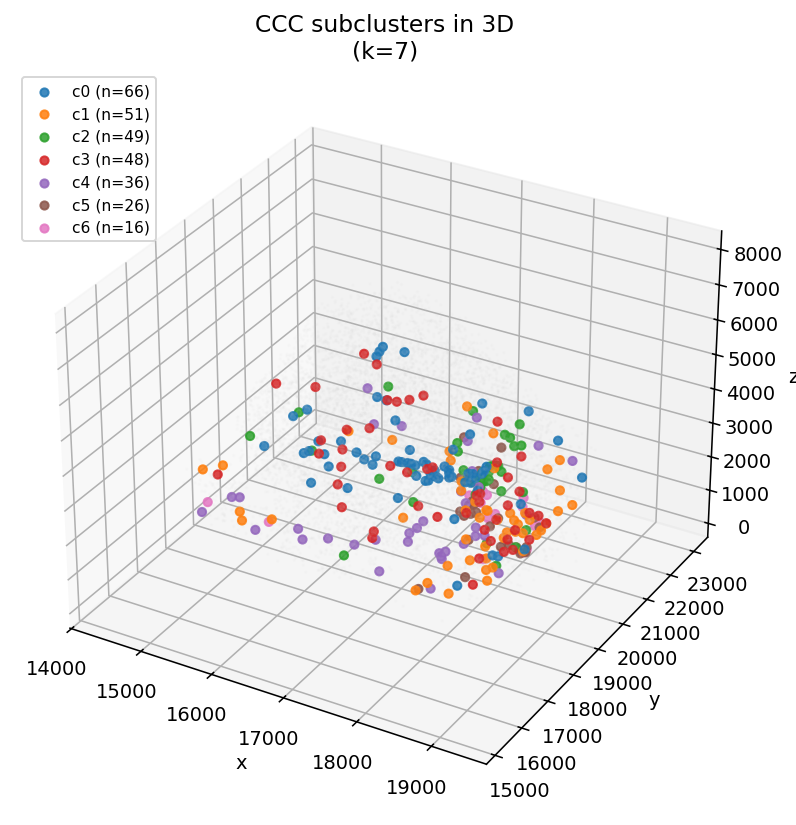
\includegraphics[width=\linewidth]{F4b_ccc_3d.png}
\caption{3D anatomical position of CCC subclusters.}
\end{subfigure}\\[0.4em]
\begin{subfigure}[t]{0.62\linewidth}
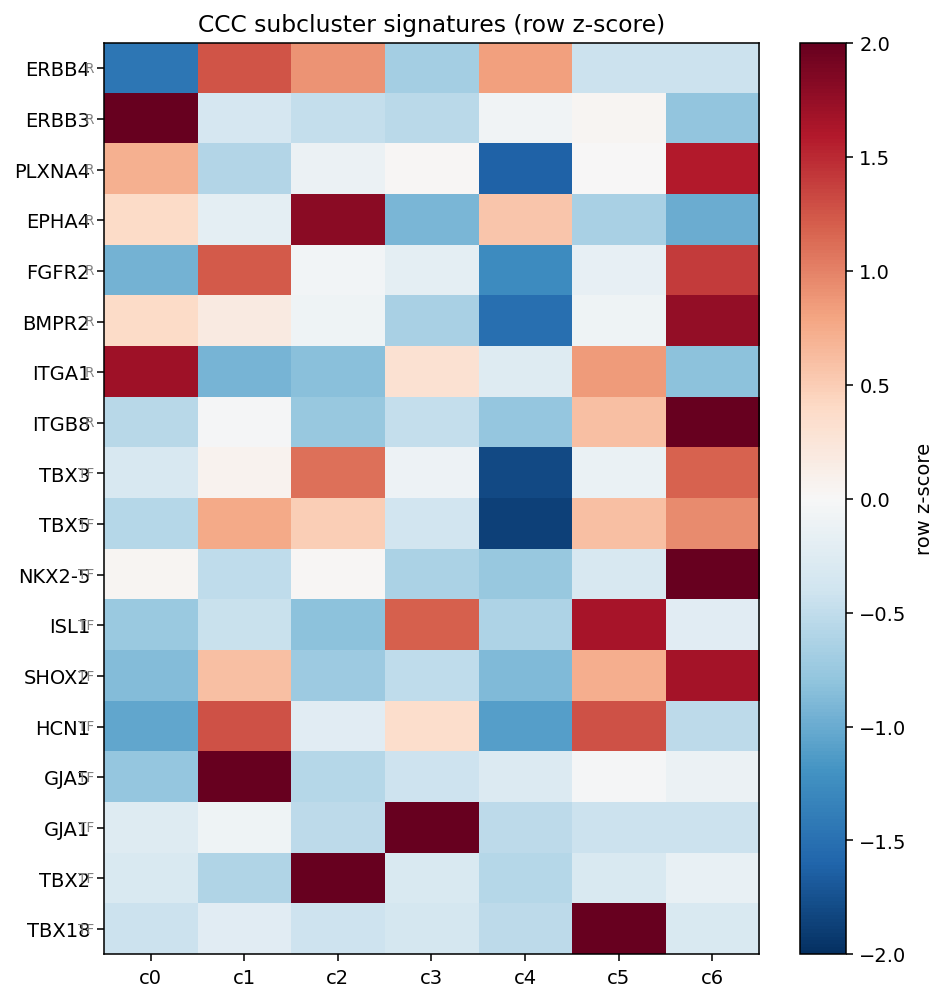
\includegraphics[width=\linewidth]{F4c_ccc_heatmap.png}
\caption{Mean-expression heatmap of receptors and CCS TFs across the
seven subclusters.}
\end{subfigure}
\caption{\textbf{CCC heterogeneity reveals canonical CCS subtypes.}
Leiden clustering on the receptor + CCS-TF panel resolves
AV-node-like (c2), SAN-like (c6), TBX18$^+$ (c5), pacemaker (c1) and
transitional (c3) subsets within the 292-cell pool.}
\label{fig:f4}
\end{figure}

\subsection{Atrial paracrine input is anti-correlated with CCS-TF
expression: a niche-driven maturation gradient}
\label{sec:gradient}

To ask whether ACM-derived signalling input correlates with the
molecular state of CCC, we computed a per-CCC \emph{niche score} for
each of the two candidate ligands (NRG3, SEMA3A) as the mean ligand
expression over the 10 nearest ACM neighbours in 3D. Niche scores were
then Spearman-correlated against each of the 10 CCS transcription
factors, with multiple-testing correction by the Benjamini--Hochberg
procedure~\citep{benjamini1995fdr} over 20 tests
(Figure~\ref{fig:f5}a, Table~\ref{tab:niche}).

Strikingly, all significant correlations point in the same direction:
\textbf{negative}. Nine of ten SEMA3A--TF and four of ten NRG3--TF
correlations were significant; in every significant case CCC cells
exposed to higher ACM-derived ligand input expressed \emph{lower}
levels of CCS transcription factors. The strongest single signal was
SEMA3A$\to$NKX2-5 ($\rho{=}-0.296$, FDR ${=}5\times 10^{-6}$), followed
by NRG3$\to$NKX2-5 ($\rho{=}-0.254$, FDR $=10^{-4}$). Quartile boxplots
of NKX2-5 expression as a function of niche-score quartile show a
clean, monotonic decrease for both ligands
(Figure~\ref{fig:f5}b).

\begin{table}[H]
\centering
\caption{Top niche-score $\to$ CCS-TF correlations
(Spearman $\rho$, BH-FDR over 20 tests).}
\label{tab:niche}
\small
\begin{tabular}{llrr}
\toprule
Ligand niche & TF & $\rho$ & FDR \\
\midrule
SEMA3A & NKX2-5 & $-0.296$ & $5\times 10^{-6}$ \\
SEMA3A & TBX18  & $-0.236$ & $3\times 10^{-4}$ \\
SEMA3A & TBX5   & $-0.225$ & $5\times 10^{-4}$ \\
SEMA3A & SHOX2  & $-0.212$ & $9\times 10^{-4}$ \\
SEMA3A & TBX3   & $-0.197$ & $2\times 10^{-3}$ \\
NRG3   & NKX2-5 & $-0.254$ & $10^{-4}$ \\
NRG3   & TBX3   & $-0.219$ & $6\times 10^{-4}$ \\
NRG3   & TBX2   & $-0.202$ & $2\times 10^{-3}$ \\
\bottomrule
\end{tabular}
\end{table}

Combined with the spatial validation of Section~\ref{sec:nrg3erbb4} ---
where the same niche-proximal CCC are also ERBB4-high --- the data
support a coherent two-axis model: \textbf{ACM-proximal CCC are
ERBB4$\uparrow$ but CCS-TF$\downarrow$ (responder / less-differentiated),
whereas ACM-distal CCC are ERBB4$\downarrow$ but CCS-TF$\uparrow$
(specified / more mature)}. Atrial NRG/SEMA input thus appears to
sustain a less-differentiated CCC pool, while specified pacemaker (c1,
c6), AV-node (c2) and TBX18$^+$ (c5) cells reside further from the
source. This is consistent with neuregulin acting as a survival /
proliferation signal during CCS development rather than imposing
identity directly~\citep{rentschler2002nrg1ccs}.

\begin{figure}[!htbp]
\centering
\begin{subfigure}[t]{0.55\linewidth}
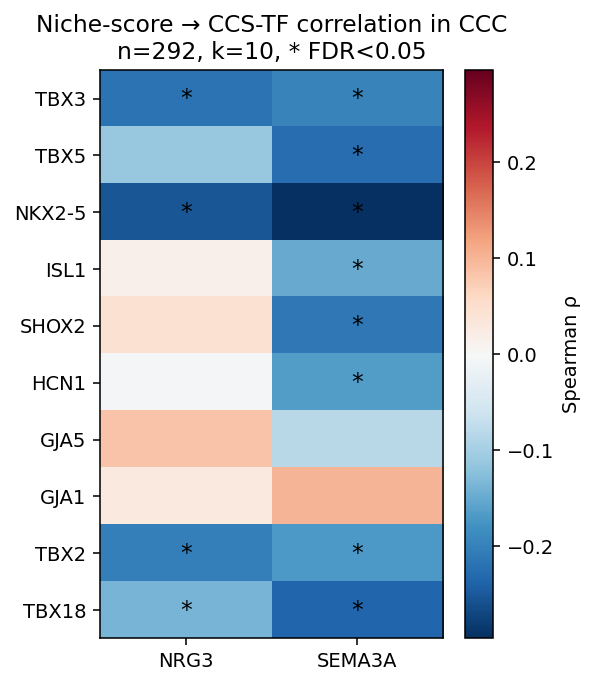
\includegraphics[width=\linewidth]{F5a_niche_tf_heatmap.png}
\caption{Spearman $\rho$ of niche-score $\to$ CCS-TF, BH-FDR-thresholded.}
\end{subfigure}\\[0.6em]
\begin{subfigure}[t]{0.85\linewidth}
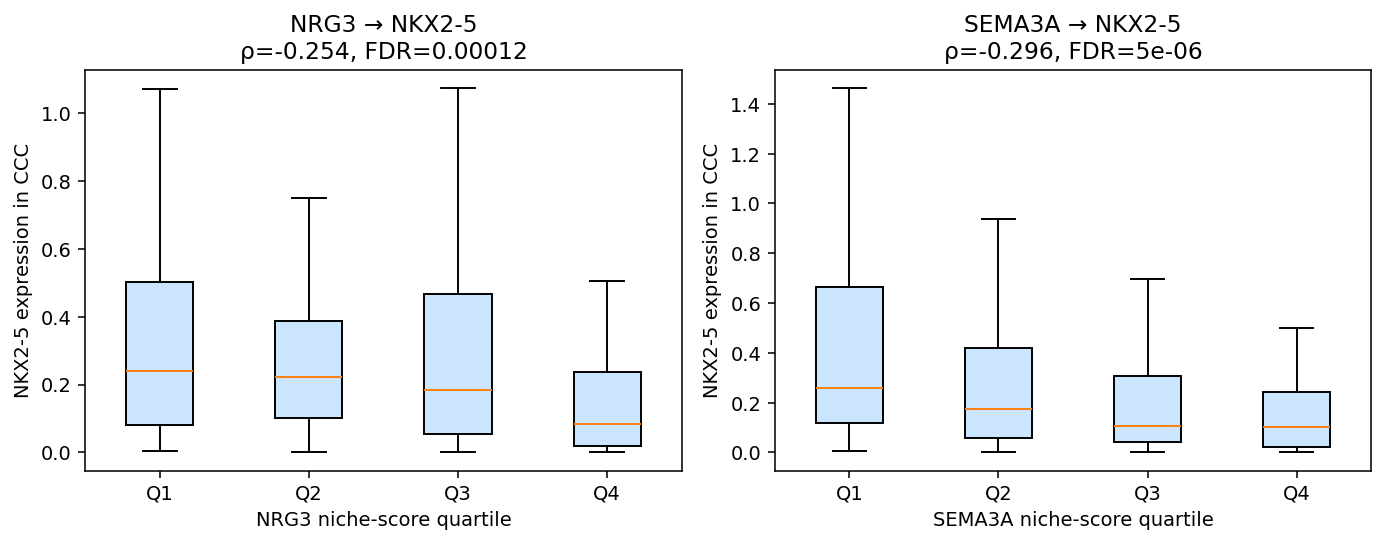
\includegraphics[width=\linewidth]{F5b_niche_quartile.png}
\caption{NKX2-5 expression in CCC across niche-score quartiles.}
\end{subfigure}
\caption{\textbf{ACM-niche scores are anti-correlated with CCS-TF
expression.} Negative correlations are systematic across both ligands;
NKX2-5 shows a clean monotonic decrease in CCC as the per-cell
NRG3/SEMA3A niche score rises.}
\label{fig:f5}
\end{figure}

% =====================================================================
\section{Discussion}

By coupling entropic optimal-transport imputation~\citep{klein2025moscot}
with 3D spatial cell--cell interaction analysis~\citep{qiu2024spateo},
we have recovered a genome-scale paracrine interactome of the human
fetal heart at PCW12 from a 238-gene MERFISH panel and used it to
formulate and test a specific developmental hypothesis: that atrial
myocardium acts as a paracrine source whose proximity correlates
inversely with conduction-system maturation.

The dominant ACM-derived signal --- NRG3$\to$ERBB4 --- is consistent
with classical genetic studies that established the requirement for
NRG/ErbB signalling in cardiac
development~\citep{lee1995erbb2,meyer1995neuregulin} and specifically
for cardiac conduction system formation in
mice~\citep{rentschler2002nrg1ccs}. Our spatial nearest-neighbour test
further demonstrates that this is a \emph{spatially coherent} signal
in human tissue, not merely a coincidence of expression: NRG3 in ACM
and ERBB4 in adjacent CCC are coupled at $\rho{=}+0.22$ against a tight
permutation null. SEMA3A's negative spatial coupling with PLXNA4 is
consistent with its established role as a repulsive guidance cue and
its requirement for normal cardiac rhythm in vivo
\citep{ieda2007sema3a}.

Within the CoreConductionCells annotation we resolved at least five
biologically interpretable subtypes (Section~\ref{sec:heterogeneity}),
including AV-node-like (TBX2$^+$/TBX3$^+$
\citep{hoogaars2007tbx3}), SAN-like (SHOX2$^+$/NKX2-5$^+$
\citep{espinozalewis2009shox2,blaschke2007shox2}) and TBX18$^+$
sinus-venosus-derived
\citep{christoffels2006tbx18,wiese2009tbx18tbx3} cells. That a
receptor + transcription-factor panel imputed from scRNA-seq onto a
target-panel MERFISH measurement is sufficient to recover canonical
CCS subtypes argues that the OT-based gene expansion preserves
biologically meaningful covariance structure, and not merely
average-state information.

Most informatively, the systematic \emph{anti}-correlation of
ACM-niche scores with CCS-TF expression
(Section~\ref{sec:gradient}) is the simplest single statement of the
data: the CCC cells closest to ACM-derived signalling are the least
differentiated cells in the conducting compartment. This is consistent
with --- though does not prove --- a model in which atrial paracrine
input sustains a proliferative, less-committed CCC pool while
specified pacemaker, AV-node and TBX18$^+$ subtypes reside further
from the ligand source. The fact that the same CCC cells that are
NRG3-niche-high are also ERBB4-high (Section~\ref{sec:nrg3erbb4})
strengthens the case that the negative TF correlation is mediated by
active receptor engagement rather than mere co-localisation.

\paragraph{Limitations.} The analysis has three principal limitations.
First, HCN4 and CNTN2, two canonical CCS markers, are not in the
5{,}187-HVG imputed set; HCN1 was used as a related substitute. A
re-run with a CCS-curated supplementary panel would refine cluster
identity, particularly for c1. Second, the seven-cluster split is on
$n{=}292$ cells; the biologically smallest clusters (c4 $n{=}36$, c6
$n{=}16$) are best treated as candidate identities rather than
statistically robust populations. Third, although CCC subclusters were
spatially intermingled in 3D, we did not formally annotate atrial vs
ventricular regions; orthogonal anatomical labels could test whether
the AV-node-like (c2) subset is enriched at the AV junction.
Confirmatory work --- in particular cross-referencing the c1/c2/c6
subtype-defining transcription factors against matching snATAC peaks
and Smart-seq2 trajectory analysis --- is a natural next step.

\paragraph{Outlook.} The pipeline established here --- an imputed
spatial atlas, a Spateo CCI loop, spatial nearest-neighbour validation
and niche-score regression --- is generalisable to other organs and
developmental stages. It does not require dedicated assays and works
with publicly available image-based spatial panels. We anticipate that
analogous gradients structure other developing-organ niches in the
human fetus.

% =====================================================================
\section{Methods}

\subsection*{Data}
The spatial atlas (\texttt{full\_heart\_final\_aug2025\_update\_downsampled\_100k.h5ad}) is a 238-gene
MERFISH measurement of the human fetal heart at PCW12, downsampled to
$10^5$ cells, with 3D coordinates in
\texttt{obsm['X\_spateo\_update']} and counts log-normalised in
\texttt{.X}. The single-cell reference
(\texttt{all\_healthy\_RoundedPCW12.h5ad}) is a 32{,}870-cell
$\times$ 31{,}019-gene scRNA-seq dataset with raw counts in
\texttt{.X} and a hierarchical \texttt{celltype} annotation
(\texttt{coarse\_celltype}, \texttt{celltype}, \texttt{celltype\_label}).
The disease gene panel comprises 247 unique heart-disease genes from
\texttt{data/heart\_disease\_genes.tsv}.

\subsection*{MOSCOT scRNA $\to$ MERFISH imputation}
Following \citet{klein2025moscot}, we used the
\texttt{moscot.problems.MappingProblem} class with
\texttt{xy\_callback="local-pca"} to compute pairwise costs. Marginals
were set asymmetric ($\tau_a{=}1$, $\tau_b{=}0.9$) to allow some
spatial cells to remain unmapped. The mapping was performed
in five non-overlapping batches of $2 \times 10^4$ spatial cells
against the full SC reference; the recovered coupling
\texttt{pi} was scaled by $n_{\text{sp}}$ before imputation. The
imputed gene set was the union of the top 5{,}000 highly variable
genes (Seurat flavour, computed on $\log_{10}(1+x)$-transformed,
size-factor-normalised SC counts via \texttt{scanpy.pp.highly\_variable\_genes})
and the 247-gene heart-disease panel, intersected with
\texttt{adata\_sc.var\_names}, yielding 5{,}187 genes (54-gene HVG--disease
overlap). Cell-cycle genes were excluded from the OT cost but retained
for imputation. Output AnnData
(\texttt{adata\_imputed\_hvg\_disease.h5ad}; 100{,}000 $\times$ 5{,}187,
4.3 GB) carries \texttt{var['is\_hvg']} and \texttt{var['is\_disease']}
flags and \texttt{obs['mapped\_celltype'/'mapped\_coarse\_celltype'/
'mapping\_confidence']}. Mean and median mapping confidence were 0.49
and 0.45 respectively.

\subsection*{Spatial cell--cell interaction analysis}
We used Spateo \citep{qiu2024spateo} to compute pairwise spatial
cell-cell interactions. After log-normalisation and a 25-nearest-neighbour
spatial graph (\texttt{spateo.tools.find\_neighbors}; $k{=}25$), we
ran \texttt{find\_cci\_two\_group} between every ordered pair of the
eight largest mapped cell types (ACM, VCM, FB, Endocardial, MuralCells,
NC, CoreConductionCells, TzConductionCells) on a 20{,}000-cell
stratified subsample, with $N_{\text{perm}}{=}10$ and
\texttt{filter\_lr="outer"}. Top-3 LR rows per ordered pair were
written to \texttt{results/cci\_hvg/all\_lr\_top3\_per\_pair.csv}.
For the conduction-cell subset (six ordered pairs centred on CCC), we
re-ran the loop with $N_{\text{perm}}{=}50$ to compensate for smaller
populations.

\subsection*{Spatial axis validation}
For each CCC cell $i$, we computed the Euclidean nearest neighbour
$j(i)$ in 3D within the ACM population and recorded the ligand
expression $L_{j(i)}$ (NRG3 or SEMA3A). We then computed the Spearman
correlation between $L_{j(i)}$ and the receptor expression $R_i$
(ERBB4 or PLXNA4) across all CCC cells. A permutation null was built
by shuffling the ACM--CCC pairing 1{,}000 times and recomputing the
correlation; the empirical $p$-value is the fraction of permuted
$|\rho|$ exceeding the observed $|\rho|$.

\subsection*{CCC subclustering}
The 292 CCC cells were extracted, $\log_{10}(1+x)$-normalised on the 18
panel features (8 receptors, 10 CCS-TFs), PCA'd to 10 components,
\texttt{scanpy.pp.neighbors} with $k{=}15$, and clustered with the
Leiden algorithm \citep{traag2019leiden} at resolution 0.8.
Cluster markers were computed across the full 5{,}187-gene set with
\texttt{scanpy.tl.rank\_genes\_groups} (Wilcoxon, BH-corrected).

\subsection*{Niche-score / TF correlation}
For each CCC cell $i$, the niche score for ligand $\ell$ was defined as
the mean of $\ell$ over the $k{=}10$ nearest ACM neighbours of $i$. We
computed the Spearman correlation between each (ligand, CCS-TF) pair
across all CCC and applied Benjamini--Hochberg
correction~\citep{benjamini1995fdr} across the 20 tests. Quartile
boxplots were generated by binning CCC cells by quartile of niche score
and plotting the distribution of TF expression.

\subsection*{Software}
Analyses were performed in Python 3.11 with
\texttt{scanpy} 1.10 \citep{wolf2018scanpy}, \texttt{moscot} 0.5.0
\citep{klein2025moscot}, \texttt{spateo} 1.1
\citep{qiu2024spateo}, \texttt{leidenalg}~\citep{traag2019leiden},
\texttt{scipy}, \texttt{numpy}, \texttt{pandas} and
\texttt{matplotlib}. All scripts and intermediate
artefacts are reproducible from
\texttt{PCW12\_analysis/scripts/\{20--28\}*}.

% =====================================================================
\section*{Data and code availability}
All analysis scripts, log files, intermediate AnnData artefacts, results
CSVs and figure source files are organised under
\texttt{PCW12\_analysis/} in the project workspace. The paper and its
LaTeX source live under \texttt{PCW12\_analysis/paper/}.

\section*{Acknowledgements}
This report was produced by the PantheonOS analysis pipeline running
locally against the project workspace. We gratefully acknowledge the
\texttt{moscot}, \texttt{spateo}, \texttt{scanpy} and
\texttt{leidenalg} development teams.

% =====================================================================
\bibliography{references}

\end{document}
